\documentclass[12pt]{article}
\usepackage{graphicx} % Required for inserting images
\usepackage[utf8]{lipsum, inputenc}
\usepackage[margin=1in]{geometry}
\usepackage{adjustbox} % for adjusting table dimensions
\usepackage{booktabs} % Used to create tables
\usepackage{tabu} % Also used to create tables
\usepackage{fancyhdr}
% \usepackage{subcaption}
\usepackage[style=chem-acs, articletitle=true]{biblatex}
\addbibresource{references.bib}
\usepackage{subfigure}


\title{Predicting Fraudulent Transaction Using Binary Classification Algorithms}
\author{Giorgos Tzimas}
\date{May 2023}

\begin{document}
\maketitle
\begin{abstract}
    Using customers' transactional dataset, we built two supervised learning machine learning algorithms, Logistic Regression and Random Forest, to classify each instance as either fraudulent or non-fraudulent transactions. After comparing the performance of both models on important metrics such as recall and False Positive Rate, we picked Random Forest as the final binary classification model to be used. 
\end{abstract}

\section{Dataset Description}
\subsection{Background}
The panel dataset contains commercial customers' financial information and days past due indicator from 2000 to 2020 provided by the Capital One Data Scientist Recruiting process. \\ \\
Dataset Link: \textbf{https://github.com/CapitalOneRecruiting/DS}

\subsection{Observations and Attributes}
The dataset comprises a comprehensive collection of \textbf{786,363} entries, encompassing \textbf{29} distinct features. These features contain a range of information pertaining to both the customer and the transactional context. Customer-related attributes include identifiers, credit card balance, credit limit, and more. Similarly, business-related attributes encompass details like business name, category, and point-of-sale information.
\vfill
\subsection{Data Types}
Out of the 29 features in the dataset:
\begin{itemize}
  \item 17 are of type "object" or text
  \item 6 are of type "integer"
  \item 3 are of type "float"
  \item 3 are of type "boolean"
\end{itemize}

\begin{table}[h!]
    \centering
    \begin{tabu}{ll}
\toprule
 & Data Type \\
Feature &  \\
\midrule
ID & int64 \\
gender & object \\
ethnicity & object \\
score & float64 \\
fcollege & object \\
mcollege & object \\
home & object \\
urban & object \\
\bottomrule
\end{tabu}
    \begin{tabu}{ll}
\toprule
 & Data Type \\
Feature &  \\
\midrule
unemp & float64 \\
wage & float64 \\
distance & float64 \\
tuition & float64 \\
education & int64 \\
income & object \\
region & object \\
\bottomrule
\end{tabu}
    \caption{Dataset attributes and their types}
    \label{tab:dtypes}
\end{table}

\section{Data Cleaning}
Some of our features are missing values either due to not being entered or that feature containing sensitive information. Features  \textbf{recurringAuthInd}, \textbf{posOnPremises}, \textbf{merchantZip}, \textbf{merchantState}, \textbf{merchantCity} and \textbf{echoBuffer} will be removed from the dataset. The rest of the features with missing values will be imputed using a "most frequent" approach due to all of them being categorical in nature.
\begin{table}[h]
    \centering
    \begin{tabu}{lr}
\toprule
 & total\_missing \\
\midrule
recurringAuthInd & 786363 \\
posOnPremises & 786363 \\
merchantZip & 786363 \\
merchantState & 786363 \\
merchantCity & 786363 \\
echoBuffer & 786363 \\
acqCountry & 4562 \\
posEntryMode & 4054 \\
merchantCountryCode & 724 \\
transactionType & 698 \\
posConditionCode & 409 \\
\bottomrule
\end{tabu}
    \caption{Features with missing values}
    \label{tab:missing}
\end{table}
\newpage
\section{Feature Extraction}
There are three datetime features in the dataset: \textbf{transactionDateTime}, \textbf{accountOpenDate}, \textbf{dateOfLastAddressChange} and \textbf{currentExpDate}. We can extract transactional information from these features to include in the dataset.\\

\noindent From \textbf{transactionDateTime}, we can get the month, day and hour that the transaction occurred.
\begin{table}[h]
    \centering
    \begin{tabu}{llrll}
\toprule
 & transactionDateTime & trans\_month & trans\_day\_name & trans\_hour \\
\midrule
0 & 2016-08-13 14:27:32 & 8 & Saturday & 14 \\
1 & 2016-10-11 05:05:54 & 10 & Tuesday & 05 \\
2 & 2016-11-08 09:18:39 & 11 & Tuesday & 09 \\
3 & 2016-12-10 02:14:50 & 12 & Saturday & 02 \\
4 & 2016-03-24 21:04:46 & 3 & Thursday & 21 \\
\bottomrule
\end{tabu}
    \caption{Features extracted from transactionDateTime}
    \label{tab:my_label}
\end{table}

\noindent Additionally, we can get the month and year from the expiration date.
\begin{table}[h]
    \centering
    \begin{tabu}{llrr}
\toprule
 & currentExpDate & exp\_month & exp\_year \\
\midrule
0 & 2023-06-01 00:00:00 & 6 & 2023 \\
1 & 2024-02-01 00:00:00 & 2 & 2024 \\
2 & 2025-08-01 00:00:00 & 8 & 2025 \\
3 & 2025-08-01 00:00:00 & 8 & 2025 \\
4 & 2029-10-01 00:00:00 & 10 & 2029 \\
\bottomrule
\end{tabu}
    \caption{Features extracted from currentExpDate}
    \label{tab:my_label}
\end{table}

\newpage
We can also extract date differences in days from each datetime feature, such as how long the account had been active, how many days since the last address change and how close to the expiration date the account was at the time of the transaction.

\begin{table}[h]
    \centering
    \resizebox{\textwidth}{!}{%
    \begin{tabu}{llllrrr}
\toprule
 & transactionDateTime & dateOfLastAddressChange & accountOpenDate & trans\_day\_addr\_change\_diff & trans\_day\_open\_date\_diff & exp\_trans\_day\_diff \\
\midrule
0 & 2016-08-13 14:27:32 & 2015-03-14 00:00:00 & 2015-03-14 00:00:00 & 518 & 518 & 2482 \\
1 & 2016-10-11 05:05:54 & 2015-03-14 00:00:00 & 2015-03-14 00:00:00 & 577 & 577 & 2668 \\
2 & 2016-11-08 09:18:39 & 2015-03-14 00:00:00 & 2015-03-14 00:00:00 & 605 & 605 & 3187 \\
3 & 2016-12-10 02:14:50 & 2015-03-14 00:00:00 & 2015-03-14 00:00:00 & 637 & 637 & 3155 \\
4 & 2016-03-24 21:04:46 & 2015-08-06 00:00:00 & 2015-08-06 00:00:00 & 231 & 231 & 4938 \\
\bottomrule
\end{tabu} }
    \caption{Date differences extracted}
    \label{tab:my_label}
\end{table}

Another feature which might be useful is whether the credit card's CVV code matched the entered CVV at the time of the transaction.

\begin{table}[h]
    \centering
    \begin{tabu}{lrrr}
\toprule
 & cardCVV & enteredCVV & matchingCVV \\
\midrule
0 & 414 & 414 & True \\
1 & 486 & 486 & True \\
2 & 486 & 486 & True \\
3 & 486 & 486 & True \\
4 & 885 & 885 & True \\
\bottomrule
\end{tabu}
    \caption{Caption}
    \label{tab:my_label}
\end{table}

The last feature to be extracted is the brand name from the merchant feature allowing us to view which store brands have the largest fraudulent transaction counts.

\begin{table}[h]
    \centering
    \begin{tabu}{lll}
\toprule
 & merchantName & brandName \\
\midrule
0 & Uber & Uber \\
1 & AMC #191138 & AMC \\
2 & Play Store & Play Store \\
3 & Play Store & Play Store \\
4 & Tim Hortons #947751 & Tim Hortons \\
5 & In-N-Out #422833 & In-N-Out \\
6 & Krispy Kreme #685312 & Krispy Kreme \\
7 & Shake Shack #968081 & Shake Shack \\
8 & Burger King #486122 & Burger King \\
9 & Five Guys #510989 & Five Guys \\
\bottomrule
\end{tabu}
    \caption{Brand name extracted from merchant feature}
    \label{tab:merchant_brand_table}
\end{table}

\newpage
\section{Exploratory Data Analysis}
In this section, we will visually explore our dataset to gain some insight into the relationships between different features.
\subsection{Total Counts by Fraud Status}
Approximately 98\% of the records are non-fraudulent. This is a very large dataset imbalance which might heavily skew the results of the model. This imbalance will be addressed with an under-sampling method during the model creation stage.
\begin{figure}[h]
    \centering
    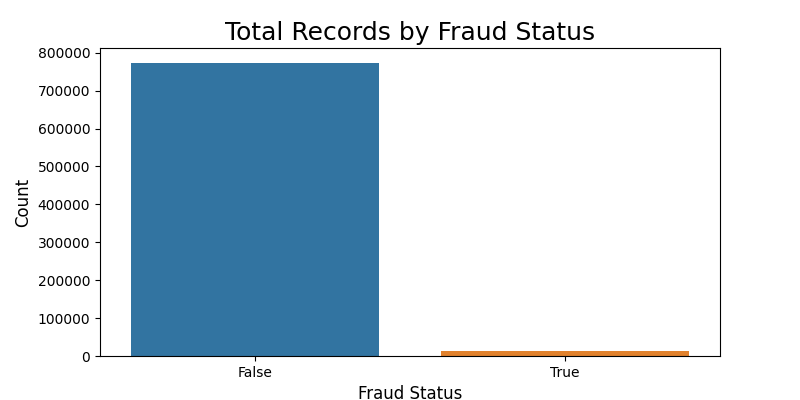
\includegraphics[width=\textwidth]{images/isFraud_counts.png}
    \caption{Caption}
    \label{fig:isFraud_counts}
\end{figure}
\newpage
\subsection{Numeric Feature Distribution}
All of the numerical features of the dataset have a right-skewed distribution. Although some of these extreme values could be outliers, it is possible that they are valid due to fraudulent transactions differing from non-fraudulent ones on a bigger scale.
\begin{figure}[h]
    \centering
    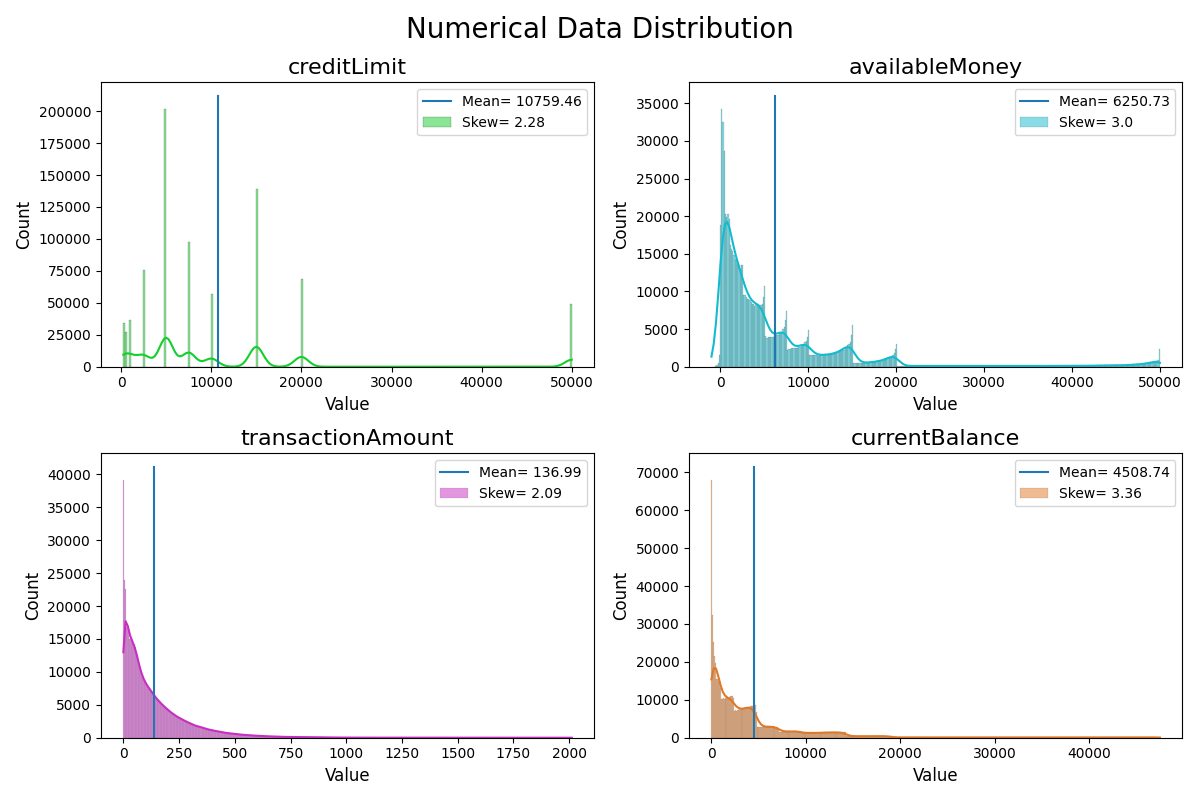
\includegraphics[width=\textwidth]{images/numeric_histograms.png}
    \caption{Distributions and mean values of numerical features}
    \label{fig:numeric_histograms}
\end{figure}

\subsection{Numeric Feature Boxplot by Fraud Status}
The biggest difference in numeric feature distributions when grouped by fraud status is visible for transaction amount. Median transaction amount is larger for fraudulent transactions compared to non-fraudulent. The interquartile range  is also larger for fraudulent transactions.
\begin{figure}[h]
    \centering
    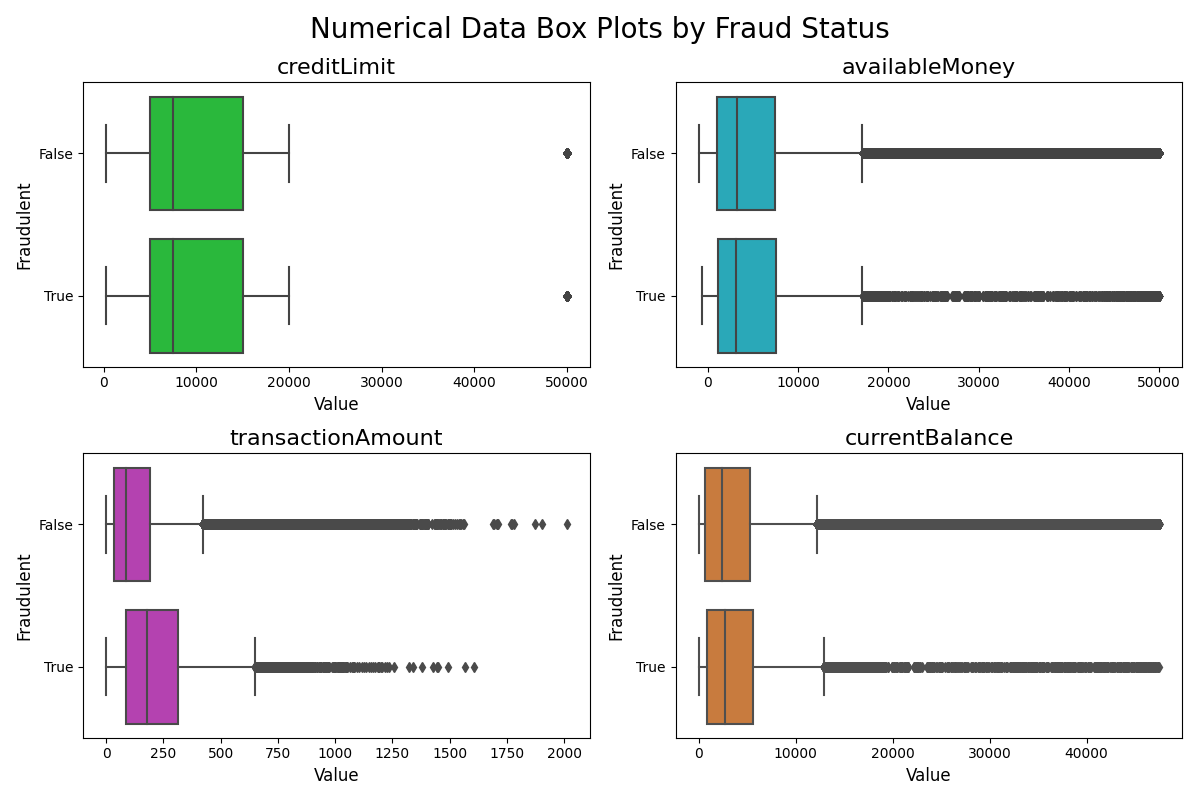
\includegraphics[width=\textwidth]{images/numeric_boxplots_by_fraud.png}
    \caption{Numeric feature boxplots by fraud status}
    \label{fig:my_label}
\end{figure}

\newpage
\subsection{Transaction Amount by Fraud Status}
The median transaction amount for fraudulent transactions is approximately \$176. For non-fraudulent transactions it is approximately \$86. Fraudulent transactions tend to cost almost double the amount of non-fraudulent ones in dollars.
\begin{figure}[h]
    \centering
    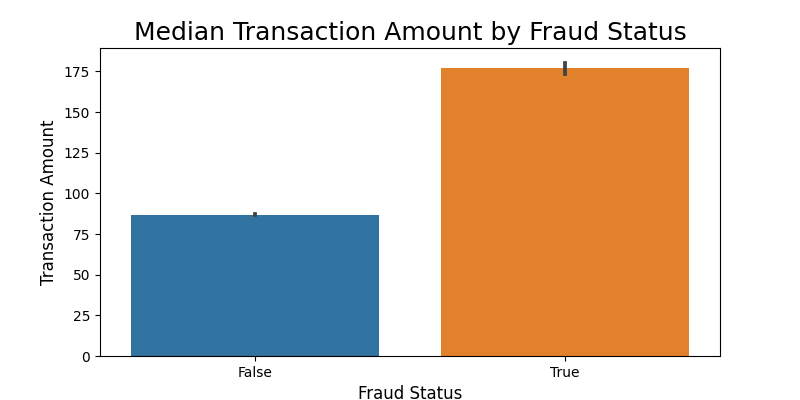
\includegraphics[width=\textwidth]{images/trans_amount_by_fraud.png}
    \caption{Median transaction amount by fraud status}
    \label{fig:my_label}
\end{figure}

\newpage
\subsection{Transactions by Country}
Approximately 99\% of the transactions in the dataset are made inside the United States. When broken down into percentages by fraud status and by country, there does not seem to be any significant difference in proportions.

\begin{figure}[h!]
    \centering
    \subfigure[Transaction count by country]{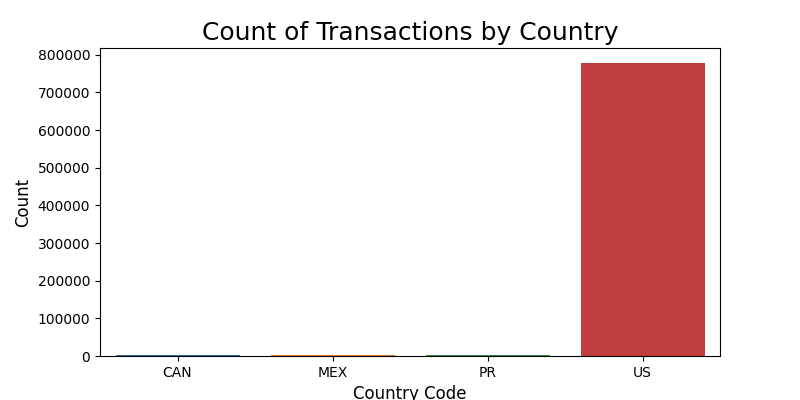
\includegraphics[width=1\textwidth]{images/trans_count_by_country.png}}
    \vspace{\baselineskip}
    \subfigure[Transaction type percentages by country]{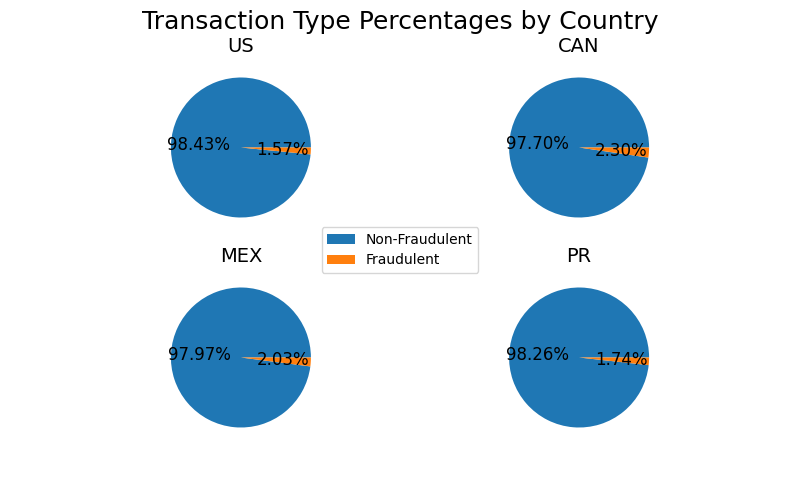
\includegraphics[width=1\textwidth]{images/trans_perc_by_country.png}}
    \label{fig:side-by-side}
    \caption{Transaction counts and proportions by status}
\end{figure}
   


\newpage
\subsection{Fraudulent Transaction Amount by Country}
Canada is the country with the largest median fraudulent transaction amount (\$229), followed by Puerto Rico (\$198), the United States (\$176) and Mexico (\$162).

\begin{figure}[h]
    \centering
    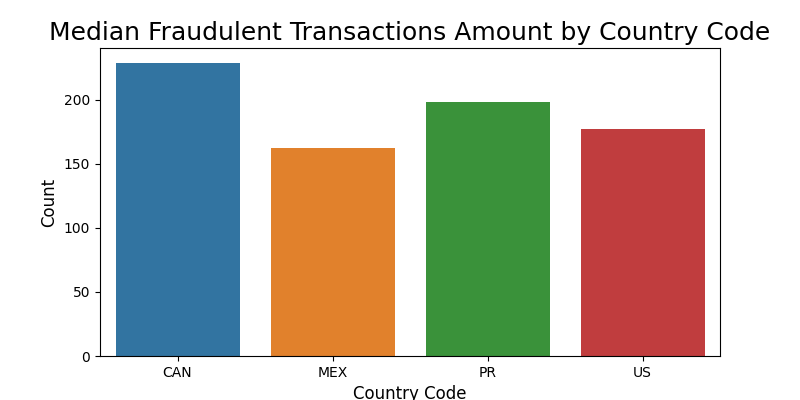
\includegraphics[width=\textwidth]{images/median_fraud_trans_amount_by_country.png}
    \caption{Median fraudulent transaction amount by country code}
    \label{fig:my_label}
\end{figure}


\subsection{Transactions by Card Presence}
There is a great difference in count of transactions by card presence when separated by fraud status. Fraudulent transactions tend to not have the credit card present at the time, presumably due to most of them occurring online where the credit card information can be inputted manually.

\begin{figure}[h!]
    \centering
    \subfigure[Transaction count by card presence and fraud status]{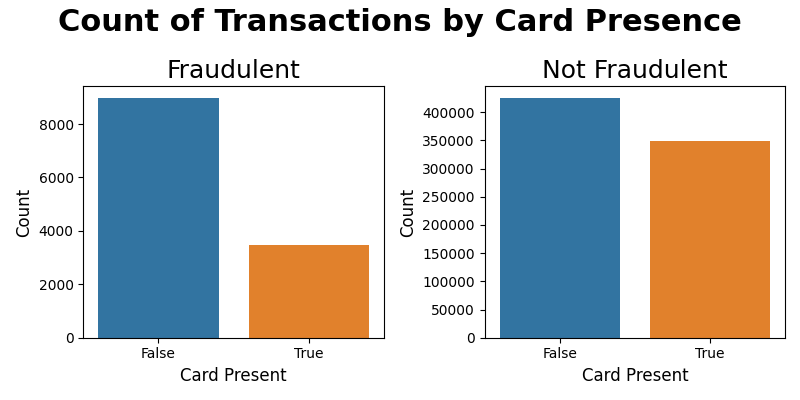
\includegraphics[width=1\textwidth]{images/count_cardPresent_by_isFraud.png}}
    \vspace{\baselineskip}
    \subfigure[Card presence percentages by fraud status]{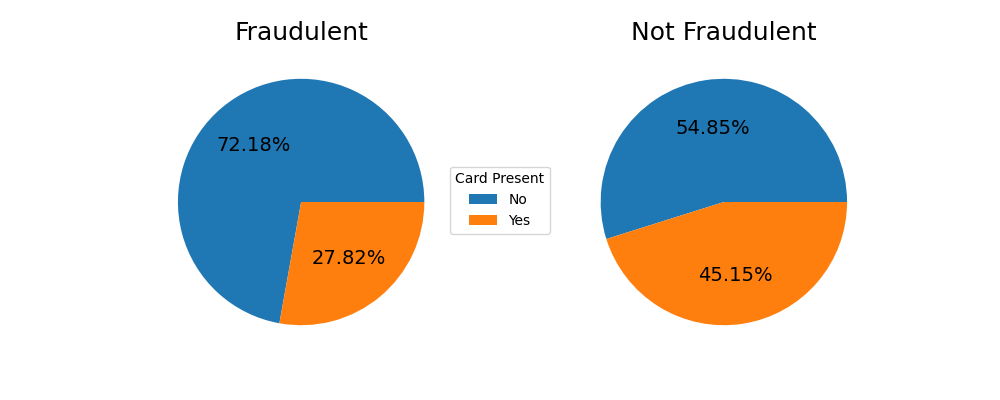
\includegraphics[width=1\textwidth]{images/perc_cardPresent_by_isFraud.png}}
    \label{fig:side-by-side}
    \caption{Transaction counts and proportions by status}
\end{figure}


\newpage
\subsection{Top 20 Brands by Transaction Count}
The brand with the most transactions in the dataset is \textbf{AMC} with 37,942 total transactions. 
\begin{figure}[h]
    \centering
    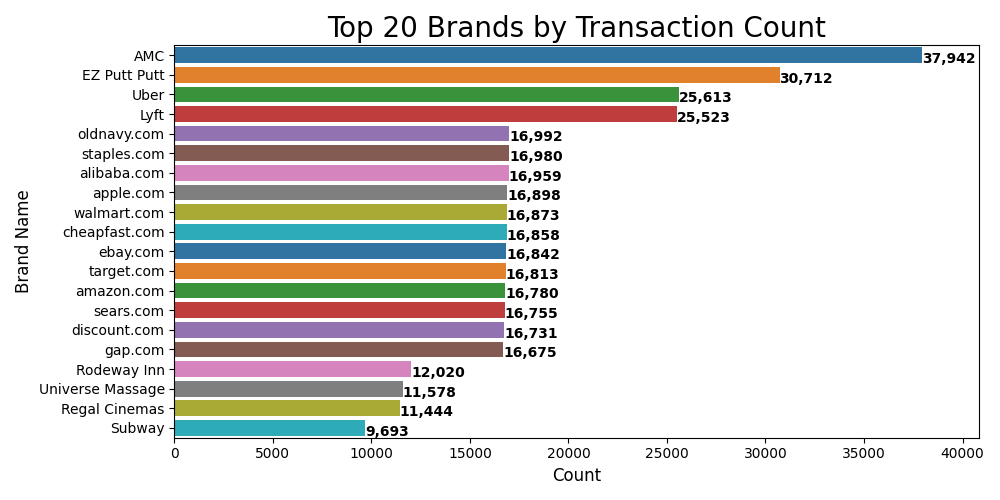
\includegraphics[width=\textwidth]{images/top_20_merchants_by_count.png}
    \caption{Top 20 brand by number of total transactions}
    \label{fig:my_label}
\end{figure}

\newpage
\subsection{Top 20 Brands by Fraudulent Transaction Count}
The brand with the most fraudulent transactions in the dataset is \textbf{Lyft} with 760 total transactions. 

\begin{figure}[h]
    \centering
    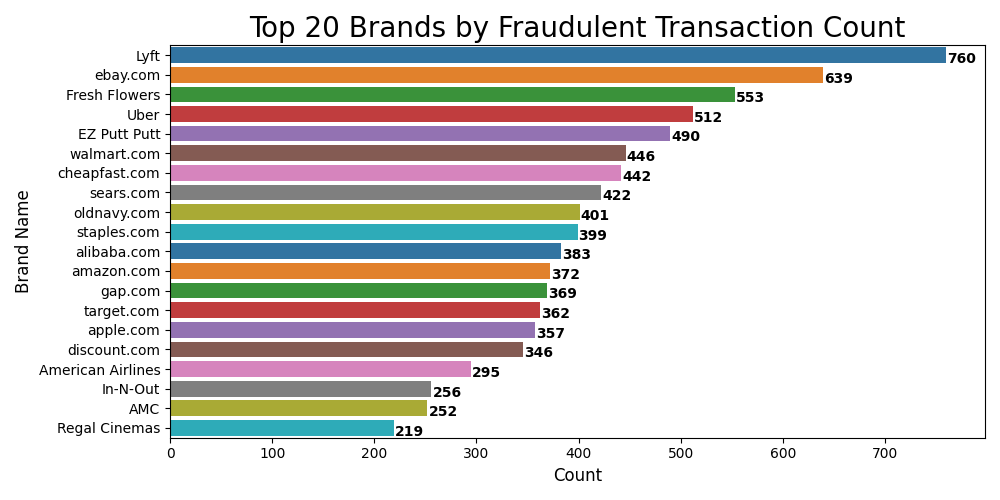
\includegraphics[width=\textwidth]{images/top_20_merchants_by_fraudulent_count.png}
    \caption{Top 20 brand by number of total fraudulent transactions}
    \label{fig:my_label}
\end{figure}

\newpage
\subsection{Top 20 Brands by Average Fraudulent Transaction Amount}
Marriott Hotels has the largest average fraudulent transaction amount at \$444.10
\begin{figure}[h]
    \centering
    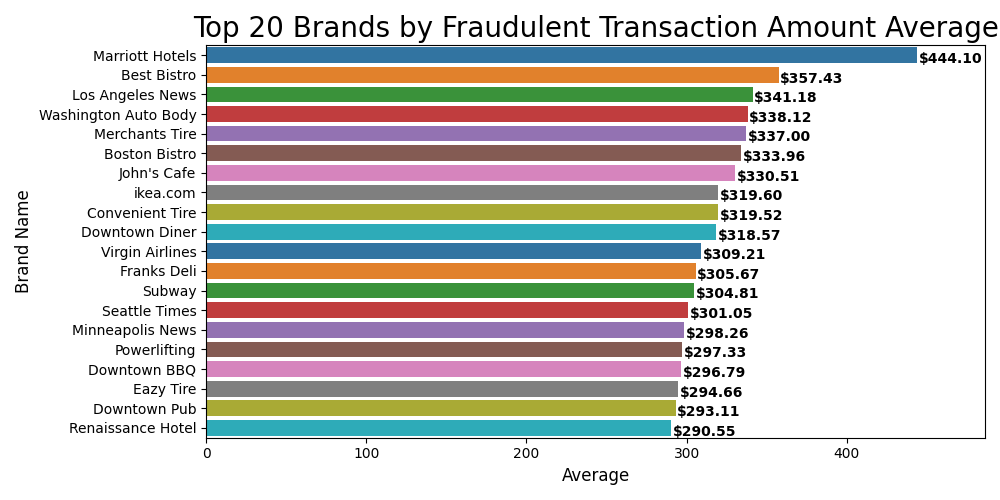
\includegraphics[width=\textwidth]{images/top_20_merchants_by_avg_trans_amount.png}
    \caption{Top 20 brand by average fraudulent transaction amount}
    \label{fig:my_label}
\end{figure}

\newpage
\section{Unsupervised Learning}
In this section we will extract patterns and structures from the dataset by grouping data points into clusters based on their inherent characteristics, enabling the discovery of natural groupings within the dataset.

\subsection{Dimensionality Reduction: Singular Value Decomposition}
Our preprocessed and transformed dataset has a total of 266 features. In order to more effectively cluster all these data points, we will perform dimensionality reduction using scikit-learn's \textbf{TruncatedSVD}, a dimensionality reduction technique commonly used in machine learning and data analysis that is particularly effective when dealing with high-dimensional data. The total number of dimenionally-reduced components for the model will be decided using the total explained variance ratio, a metric used to assess the amount of information or variability in the data.

\begin{figure}[h]
    \centering
    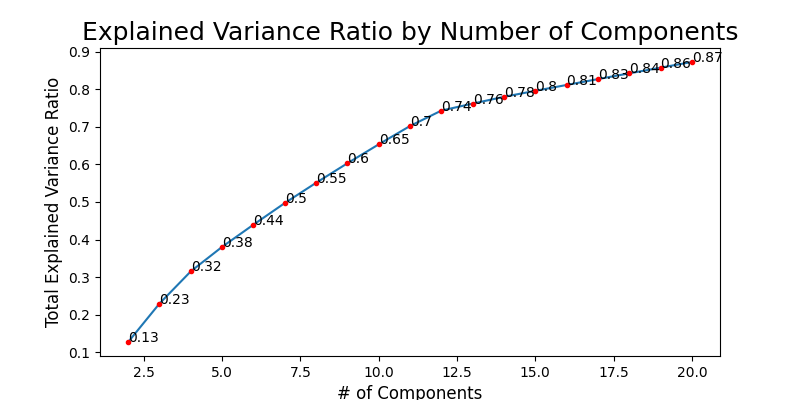
\includegraphics[width=\textwidth]{images/explained_variance_ratio.png}
    \caption{Total Explained Variance Ratio based on number of components}
    \label{fig:my_label}
\end{figure}
With 12 components we can retain approximately 74\% of the variance of the original dataset. In addition, we drastically reduced the number of features from 266 to only 12.

\newpage
\subsection{Clustering: KMeans}
With our dimensionally-reduced dataset, we will build a KMeans clustering model to group those datapoints. The optimal number of clusters will be determined by calculating the within-cluster sum of squares for the model, a metric used in K-means clustering to evaluate the quality of the clustering solution.

\begin{figure}[h]
    \centering
    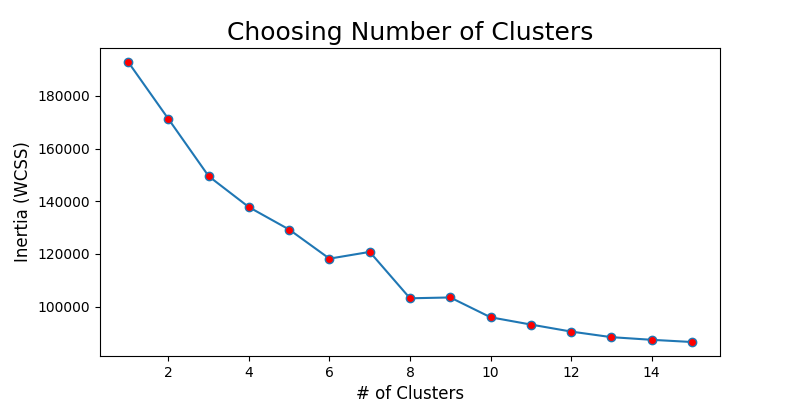
\includegraphics[width=\textwidth]{images/kmeans_inertia.png}
    \caption{Within-Cluster Sum of Squares based on number of clusters}
    \label{fig:my_label}
\end{figure}
\newpage
We will use 4 clusters for the KMeans algorithm, with a total within-cluster sum of squares of 140,216.
\begin{figure}[h]
    \centering
    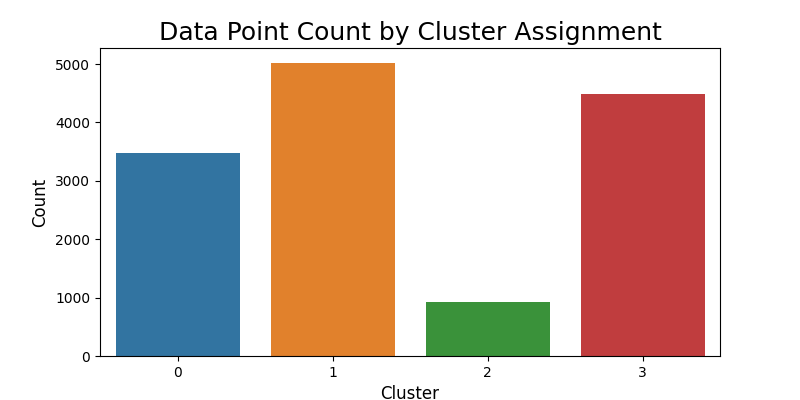
\includegraphics[width=1\textwidth]{images/count_by_cluster.png}
    \caption{Caption}
    \label{fig:my_label}
\end{figure}
\newpage
Cluster 1 has the largest count of data points, followed by cluster 3, cluster 0 and cluster 2.

\section{Supervised Learning}
Supervised learning is a machine learning approach where a model learns to make predictions or decisions based on labeled training data. In supervised learning, we have a dataset consisting of input features and corresponding target labels or outputs. The goal is to train a model that can generalize from the provided examples and accurately predict the target labels for new, unseen data. We will create two different machine learning model to classify the data as fraudulent or non-fraudulent.

\subsection{Dataset Resampling}
Due to our dependent variable being drastically imbalanced, we will need to resample the dataset to eliminate that imbalance. Since our minority class contains 12,417 records, we will use under-sampling, which is a method that aims to reduce the imbalance between classes by randomly removing samples from the majority class until the desired balance is achieved.

\begin{table}[h]
    \centering
    \begin{tabu}{lrr}
\toprule
 & Original & Under-Sampled \\
isFraud &  &  \\
\midrule
False & 773946 & 12417 \\
True & 12417 & 12417 \\
\bottomrule
\end{tabu}
    \caption{Transaction by fraud status before and after resampling}
    \label{tab:my_label}
\end{table}
\newpage
Now both fraudulent and non-fraudulent transactions are equal in count, which will significantly increase our model performances.

\subsection{Hyperparameter Tuning}
For both the Logistic Regression and Random Forest models, hyperparameter estimation and tuning will be done using scikit-learn's \textbf{GridSearchCV}. GridSearchCV systematically searches and evaluates the performance of a model across a grid of possible hyperparameter values and returns the best-tuned model that will yield the greatest performance.


\begin{figure}[h]
    \centering
    \subfigure[Logistic Regression]{
        \begin{tabu}{lll}
\toprule
 & param & value \\
\midrule
0 & C & 0.500000 \\
1 & class\_weight & NaN \\
2 & dual & False \\
3 & fit\_intercept & True \\
4 & intercept\_scaling & 1 \\
5 & l1\_ratio & NaN \\
6 & max\_iter & 500 \\
7 & multi\_class & auto \\
8 & n\_jobs & NaN \\
9 & penalty & l1 \\
10 & random\_state & NaN \\
11 & solver & saga \\
12 & tol & 0.000100 \\
13 & verbose & 0 \\
14 & warm\_start & False \\
\bottomrule
\end{tabu}
        \label{subfig:table1}
    }
    \hfill
    \subfigure[Random Forest]{
        \begin{tabu}{lll}
\toprule
 & param & value \\
\midrule
0 & bootstrap & True \\
1 & ccp\_alpha & 0.000000 \\
2 & class\_weight & NaN \\
3 & criterion & gini \\
4 & max\_depth & 5 \\
5 & max\_features & auto \\
6 & max\_leaf\_nodes & NaN \\
7 & max\_samples & NaN \\
8 & min\_impurity\_decrease & 0.000000 \\
9 & min\_samples\_leaf & 4 \\
10 & min\_samples\_split & 2 \\
11 & min\_weight\_fraction\_leaf & 0.000000 \\
12 & n\_estimators & 100 \\
13 & n\_jobs & NaN \\
14 & oob\_score & True \\
15 & random\_state & NaN \\
16 & verbose & 0 \\
17 & warm\_start & False \\
\bottomrule
\end{tabu}
        \label{subfig:table2}
    }
    \caption{Hyperparameters for both models}
    \label{fig:tables}
\end{figure}

\newpage
\subsection{Logistic Regression}
Logistic Regression models the relationship between the input features and the probability of belonging to a particular class.  The input features are linearly combined with weights or coefficients, and then passed through a sigmoid or logistic function. The sigmoid function maps the linear combination to a value between 0 and 1, representing the probability of the input belonging to the positive class. \\

\noindent Using the best estimator result from GridSearchCV, we fit the training and testing dataset to the model and get the probabilities for the positive class. We then compute the ROC-AUC Curve to find the most appropriate threshold value for the model.
\begin{figure}[h]
    \centering
    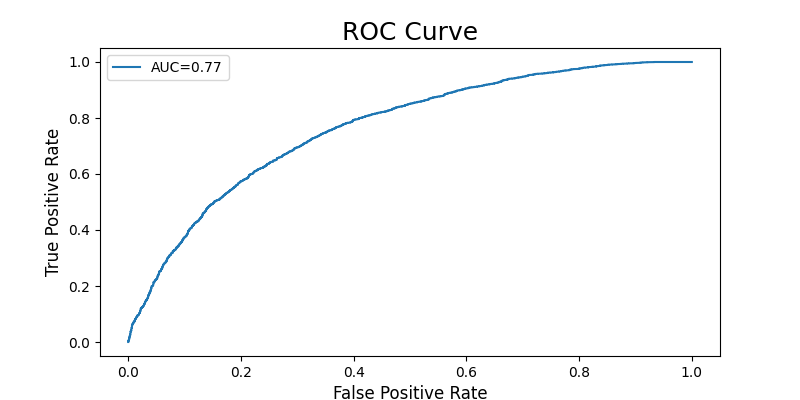
\includegraphics[width=\textwidth]{images/roc_lr.png}
    \caption{ROC-AUC curve for Logistic Regression}
    \label{fig:my_label}
\end{figure}

\begin{table}[h]
    \centering
    \begin{adjustbox}{width=1\textwidth}
    \begin{tabu}{lrrrrrrr}
\toprule
 & thresh=0.3 & thresh=0.35 & thresh=0.4 & thresh=0.45 & thresh=0.5 & thresh=0.55 & thresh=0.6 \\
\midrule
Accuracy & 0.634290 & 0.658782 & 0.679919 & 0.695689 & 0.699379 & 0.694682 & 0.683946 \\
Recall/Sensitivity & 0.930560 & 0.890641 & 0.840322 & 0.790003 & 0.729621 & 0.653137 & 0.561892 \\
False Positive Rate & 0.662081 & 0.573154 & 0.480537 & 0.398658 & 0.330872 & 0.263758 & 0.193960 \\
Precision & 0.584369 & 0.608526 & 0.636271 & 0.664691 & 0.688073 & 0.712404 & 0.743453 \\
Specificity & 0.337919 & 0.426846 & 0.519463 & 0.601342 & 0.669128 & 0.736242 & 0.806040 \\
F1 Score & 0.717909 & 0.723039 & 0.724198 & 0.721950 & 0.708238 & 0.681484 & 0.640046 \\
\bottomrule
\end{tabu}
    \end{adjustbox}{}
    \caption{Model metrics for different threshold values}
    \label{tab:my_label}
\end{table}

\noindent In our case, a threshold of 0.45 seems to yield the best results for our purpose. We want to correctly classify as many actual positive cases as possible but not at the cost of a very high False Positive rate. This threshold offers a good balance in this case, with a harmonic mean value (F1 Score) of 0.72198. 


\begin{figure}[h]
    \centering
    \subfigure[Confusion matrix]{
        \begin{tabu}{llrr}
\toprule
 &  & \multicolumn{2}{r}{Predicted} \\
 &  & 0 & 1 \\
\midrule
\multirow{Actual} & 0 & 1792 & 1188 \\
 & 1 & 626 & 2355 \\
\cline{1-4}
\bottomrule
\end{tabu}
        \label{subfig:table1}
    }
    \hspace{1cm}
    \subfigure[Model metrics]{
        \begin{tabu}{lr}
\toprule
 & thresh=0.45 \\
\midrule
Accuracy & 0.695689 \\
Recall/Sensitivity & 0.790003 \\
False Positive Rate & 0.398658 \\
Precision & 0.664691 \\
Specificity & 0.601342 \\
F1 Score & 0.721950 \\
\bottomrule
\end{tabu}
        \label{subfig:table2}
    }
    \caption{Logistic Regression results with threshold equal to 0.45}
    \label{fig:tables}
\end{figure}
\newpage
\noindent Our final Logistic Regression model has an accuracy of 0.6957, True Positive Rate of 0.79 and a False Positive Rate of 0.3987. We will cross-validate the model performance by training it 50 times to get the mean metrics, distributions and confidence intervals for each metric.

\begin{figure}[h]
    \centering
    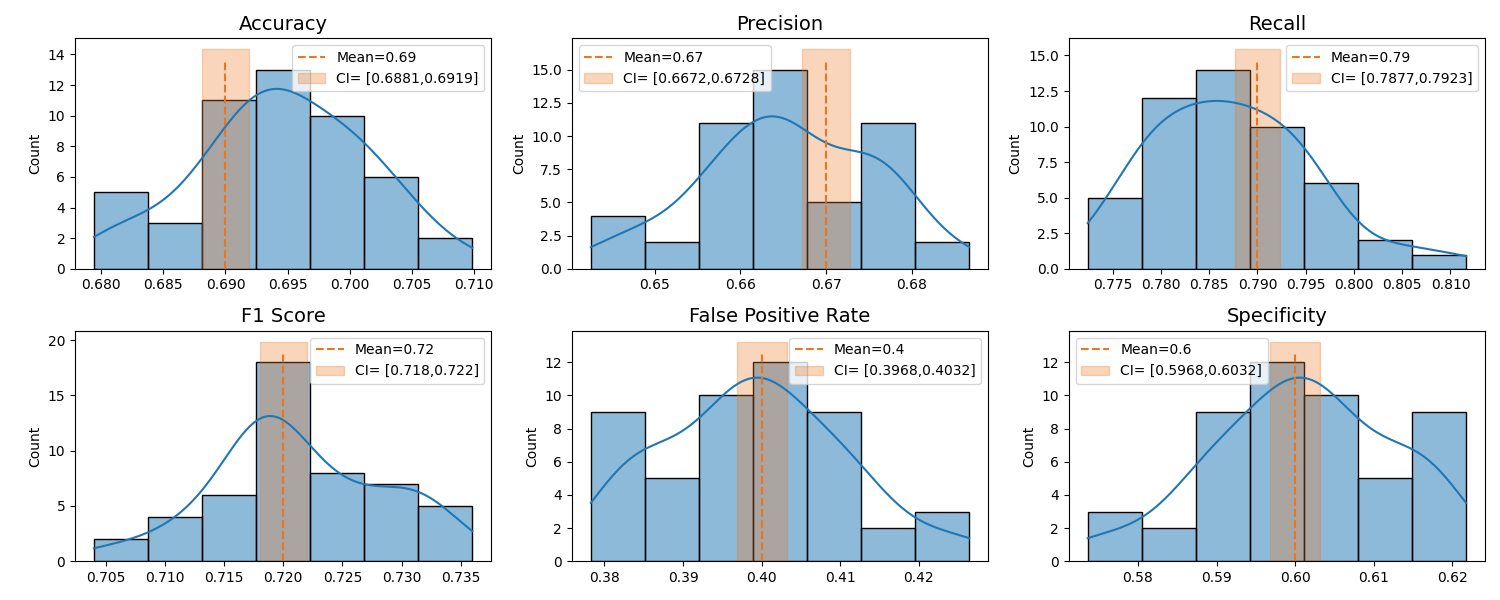
\includegraphics[width=1.15\textwidth]{images/lr_metrics_graph.png}
    \caption{Logistic Regression metrics (n\_fits=50)}
    \label{fig:my_label}
\end{figure}

\textbf{Results}:
\noindent If we were to repeat the estimation process n number of times, in 95\% of cases our metrics would fall in the following ranges:
\begin{itemize}
  \item Accuracy: [0.6881, 0.6919]
  \item Precision: [0.6672, 0.6728]
  \item Recall: [0.7877, 0.7923]
  \item F1 Score: [0.7180, 0.7220]
  \item False Positive Rate: [0.3968, 0.4032]
  \item Specificity: [0.5968, 0.6032]
\end{itemize}

\subsection{Logistic Regression Feature Importances}
In order to determine what the most important features for the Logistic Regression model are, we will look at the top 20 features with the largest absolute coefficients. The magnitude of the coefficient indicates the strength of the relationship between the independent variable and the log-odds of the event. A larger magnitude suggests a stronger influence on the outcome.

\begin{figure}[h]
    \centering
    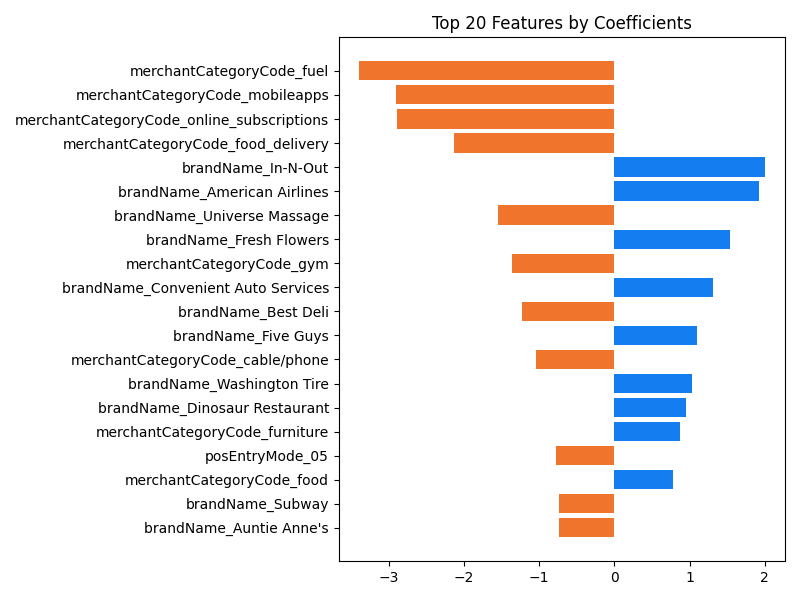
\includegraphics[width=\textwidth]{images/lr_feature_importances.png}
    \caption{Most important features for Linear Regression model}
    \label{fig:enter-label}
\end{figure}

\begin{table}[h]
    \centering
    \resizebox{0.5\textwidth}{!}{%
    \begin{tabu}{lr}
\toprule
 & Coef. \\
Feature &  \\
\midrule
merchantCategoryCode\_fuel & -3.393160 \\
merchantCategoryCode\_mobileapps & -2.907693 \\
merchantCategoryCode\_online\_subscriptions & -2.887401 \\
merchantCategoryCode\_food\_delivery & -2.127403 \\
brandName\_In-N-Out & 1.998216 \\
brandName\_American Airlines & 1.917929 \\
brandName\_Universe Massage & -1.545704 \\
brandName\_Fresh Flowers & 1.531638 \\
merchantCategoryCode\_gym & -1.364648 \\
brandName\_Convenient Auto Services & 1.311114 \\
brandName\_Best Deli & -1.224450 \\
brandName\_Five Guys & 1.104633 \\
merchantCategoryCode\_cable/phone & -1.039582 \\
brandName\_Washington Tire & 1.028438 \\
brandName\_Dinosaur Restaurant & 0.947981 \\
merchantCategoryCode\_furniture & 0.876960 \\
posEntryMode\_05 & -0.782440 \\
merchantCategoryCode\_food & 0.777277 \\
brandName\_Subway & -0.737239 \\
brandName\_Auntie Anne's & -0.730191 \\
\bottomrule
\end{tabu}
 }
    \caption{Features with largest absolute coefficients for Logistic Regression model}
    \label{tab:my_label}
\end{table}

The most important feature by coefficient effect is \textbf{merchantCategoryCode\_fuel}.
\newpage
\subsection{Random Forest}
Random Forest is an ensemble machine learning algorithm that is composed of multiple decision trees, with each tree trained independently on a random subset of the training data. The class with the most votes across all the trees is selected as the predicted class. It is less prone to overfitting and able to handle data with a large number of features, both categorical and numerical.

\noindent Same as with our Linear Regression model, we will use the best estimator resulting from GridSearchCV and fit preprocessed dataset.
\begin{figure}[h]
    \centering
    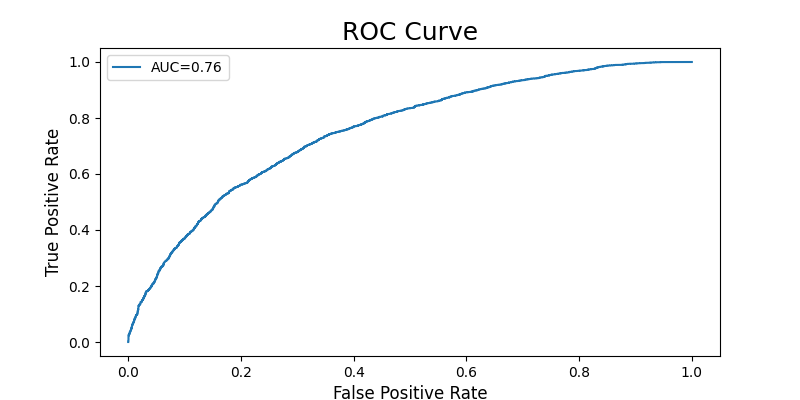
\includegraphics[width=\textwidth]{images/roc_rf.png}
    \caption{ROC-AUC curve for Random Forest}
    \label{fig:my_label}
\end{figure}

\begin{table}[h]
    \centering
    \begin{adjustbox}{width=1\textwidth}
    \begin{tabu}{lrrrrrrr}
\toprule
 & thresh=0.3 & thresh=0.35 & thresh=0.4 & thresh=0.45 & thresh=0.5 & thresh=0.55 & thresh=0.6 \\
\midrule
Accuracy & 0.517698 & 0.532293 & 0.571213 & 0.651065 & 0.687301 & 0.657608 & 0.580607 \\
Recall/Sensitivity & 1.000000 & 0.998658 & 0.969473 & 0.877893 & 0.723247 & 0.454881 & 0.210332 \\
False Positive Rate & 0.964765 & 0.934228 & 0.827181 & 0.575839 & 0.348658 & 0.139597 & 0.048993 \\
Precision & 0.509051 & 0.516751 & 0.539683 & 0.603970 & 0.674804 & 0.765237 & 0.811125 \\
Specificity & 0.035235 & 0.065772 & 0.172819 & 0.424161 & 0.651342 & 0.860403 & 0.951007 \\
F1 Score & 0.674663 & 0.681080 & 0.693378 & 0.715614 & 0.698187 & 0.570587 & 0.334044 \\
\bottomrule
\end{tabu}
    \end{adjustbox}{}
    \caption{Model metrics for different threshold values}
    \label{tab:my_label}
\end{table}
\newpage
\noindent For this model, a threshold of 0.5 seems to be the most appropriate, with a harmonic mean value (F1 Score) of 0.698187.
 

\begin{figure}[h]
    \centering
    \subfigure[Confusion matrix]{
        \begin{tabu}{llrr}
\toprule
 &  & \multicolumn{2}{r}{Predicted} \\
 &  & 0 & 1 \\
\midrule
\multirow{Actual} & 0 & 1992 & 988 \\
 & 1 & 865 & 2116 \\
\cline{1-4}
\bottomrule
\end{tabu}
        \label{subfig:table1}
    }
    \hspace{1cm}
    \subfigure[Model metrics]{
        \begin{tabu}{lr}
\toprule
 & thresh=0.5 \\
\midrule
Accuracy & 0.689146 \\
Recall/Sensitivity & 0.709829 \\
False Positive Rate & 0.331544 \\
Precision & 0.681701 \\
Specificity & 0.668456 \\
F1 Score & 0.695481 \\
\bottomrule
\end{tabu}
        \label{subfig:table2}
    }
    \caption{Random Forest results with threshold equal to 0.50}
    \label{fig:tables}
\end{figure}

\noindent Our final Random Forest model has an accuracy of 0.6891, True Positive Rate of 0.71 and a False Positive Rate of 0.33. As with the Linear Regression model, we will cross-validate the model performance by training it 50 times to get the mean metrics, distributions and confidence intervals for each metric.

\begin{figure}[h]
    \centering
    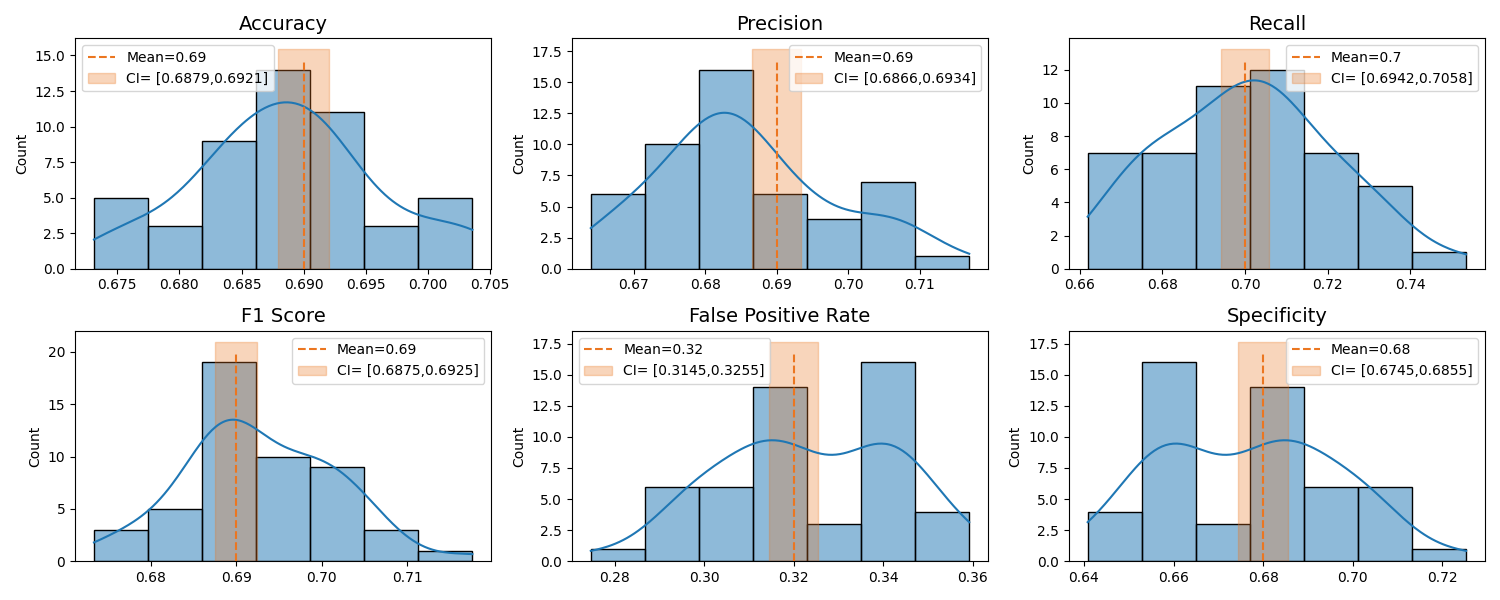
\includegraphics[width=1.15\textwidth]{images/rf_metrics_graph.png}
    \caption{Logistic Regression metrics (n\_fits=50)}
    \label{fig:my_label}
\end{figure}

\textbf{Results}:
\noindent If we were to repeat the estimation process n number of times, in 95\% of cases our metrics would fall in the following ranges:
\begin{itemize}
  \item Accuracy: [0.6879, 0.6921]
  \item Precision: [0.6866, 0.6934]
  \item Recall: [0.6942, 0.7058]
  \item F1 Score: [0.6875, 0.6925]
  \item False Positive Rate: [0.3145, 0.3255]
  \item Specificity: [0.6745, 0.6855]
\end{itemize}

\subsection{Random Forest Feature Importances}
Random Forest feature importances provide a measure of the relative importance of each feature in a Random Forest model. The feature importances are calculated based on the impurity reduction or information gain that each feature contributes to the overall performance of the Random Forest. The total sum of all values equals to 1, so each value gives us the proportion of importance in the total model.

\begin{figure}[h]
    \centering
    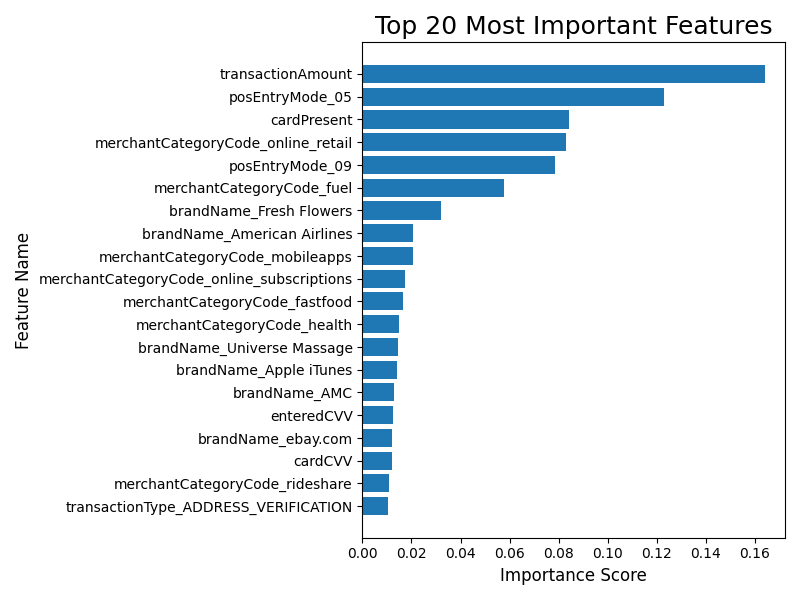
\includegraphics[width=\textwidth]{images/rf_importance_scores.png}
    \caption{Most important features for Random Forest model}
    \label{fig:enter-label}
\end{figure}
\newpage
\begin{table}[h]
    \centering
    \resizebox{0.5\textwidth}{!}{%
    \begin{tabu}{lr}
\toprule
 & Proportion \\
Feature &  \\
\midrule
transactionAmount & 0.164092 \\
posEntryMode\_05 & 0.123055 \\
cardPresent & 0.084142 \\
merchantCategoryCode\_online\_retail & 0.082937 \\
posEntryMode\_09 & 0.078340 \\
merchantCategoryCode\_fuel & 0.057539 \\
brandName\_Fresh Flowers & 0.032164 \\
brandName\_American Airlines & 0.020716 \\
merchantCategoryCode\_mobileapps & 0.020647 \\
merchantCategoryCode\_online\_subscriptions & 0.017387 \\
merchantCategoryCode\_fastfood & 0.016681 \\
merchantCategoryCode\_health & 0.014733 \\
brandName\_Universe Massage & 0.014493 \\
brandName\_Apple iTunes & 0.014050 \\
brandName\_AMC & 0.012724 \\
enteredCVV & 0.012533 \\
brandName\_ebay.com & 0.012169 \\
cardCVV & 0.011947 \\
merchantCategoryCode\_rideshare & 0.010692 \\
transactionType\_ADDRESS\_VERIFICATION & 0.010458 \\
\bottomrule
\end{tabu} }
    \caption{Features with largest importance for Random Forest model}
    \label{tab:my_label}
\end{table}

The most relevant feature in determining whether a transaction is fraudulent is \textbf{transactionAmount} (0.16), followed by \textbf{posEntryMode\_05} (0.12) and \textbf{cardPresent} (0.08).

\newpage
\section{Model Comparison}
Out of the two classification models, Random Forest seems to have the best performance for our purposes, with a recall score of 0.715137 and a False Positive Rate of 0.332624. Althouth Logistic Regression is outperforming the Random Forest model when it comes to recall, it also has a relatively high False Positive Rate in comparison. 

\begin{figure}[h]
    \centering
    \subfigure[Model metrics]{
        \begin{adjustbox}{width=1\textwidth}
    
        \begin{tabu}{lrr}
\toprule
 & Logistic Regression (thresh=0.45) & Random Forest (thresh=0.5) \\
\midrule
Accuracy & 0.691585 & 0.691048 \\
Recall/Sensitivity & 0.786623 & 0.715137 \\
False Positive Rate & 0.401809 & 0.332624 \\
Precision & 0.657984 & 0.678746 \\
Specificity & 0.598191 & 0.667376 \\
F1 Score & 0.716576 & 0.696466 \\
\bottomrule
\end{tabu}
        \end{adjustbox}{}
        \label{subfig:table1}
    }
    \hspace{1cm}
    \subfigure[ROC-AUC Curves]{
        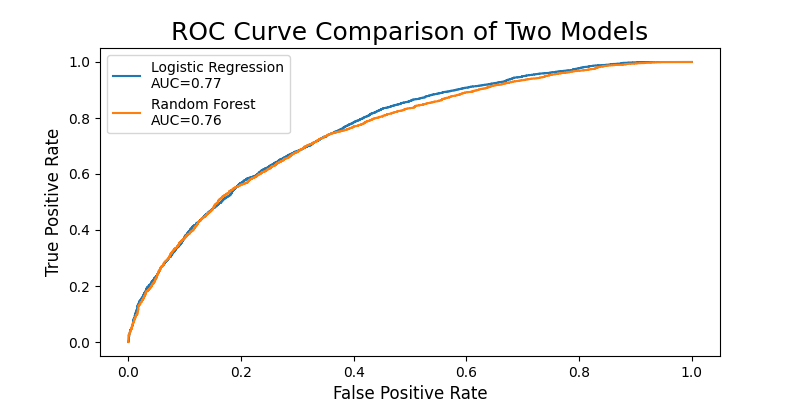
\includegraphics[width=1\textwidth]{images/roc_both_models.png}
        \label{subfig:table2}
    }
    \caption{Comparison of both classification algorithms}
    \label{fig:tables}
\end{figure}

\end{document}
